\documentclass{beamer}
\mode<presentation>{\usetheme{AV}}
\usepackage{etex}
\usepackage[export]{adjustbox}
\usepackage{epsfig}
\usepackage{feynmp}
\usepackage{verbatim}
\usepackage{listings}
\usepackage{colortbl}

\usepackage{color}

\definecolor{mygreen}{rgb}{0,0.6,0}
\definecolor{mygray}{rgb}{0.5,0.5,0.5}
\definecolor{mymauve}{rgb}{0.58,0,0.82}

\lstset{ %
  backgroundcolor=\color{white},   % choose the background color; you must add \usepackage{color} or \usepackage{xcolor}
%  basicstyle=\footnotesize,        % the size of the fonts that are used for the code
  breakatwhitespace=false,         % sets if automatic breaks should only happen at whitespace
  breaklines=true,                 % sets automatic line breaking
  captionpos=b,                    % sets the caption-position to bottom
  commentstyle=\color{mygreen},    % comment style
  deletekeywords={...},            % if you want to delete keywords from the given language
  escapeinside={\%*}{*)},          % if you want to add LaTeX within your code
  extendedchars=true,              % lets you use non-ASCII characters; for 8-bits encodings only, does not work with UTF-8
  frame=single,                    % adds a frame around the code
  keepspaces=true,                 % keeps spaces in text, useful for keeping indentation of code (possibly needs columns=flexible)
  keywordstyle=\color{blue},       % keyword style
  language=Octave,                 % the language of the code
  morekeywords={*,...},            % if you want to add more keywords to the set
  numbers=left,                    % where to put the line-numbers; possible values are (none, left, right)
  numbersep=5pt,                   % how far the line-numbers are from the code
  numberstyle=\tiny\color{mygray}, % the style that is used for the line-numbers
  rulecolor=\color{black},         % if not set, the frame-color may be changed on line-breaks within not-black text (e.g. comments (green here))
  showspaces=false,                % show spaces everywhere adding particular underscores; it overrides 'showstringspaces'
  showstringspaces=false,          % underline spaces within strings only
  showtabs=false,                  % show tabs within strings adding particular underscores
  stepnumber=2,                    % the step between two line-numbers. If it's 1, each line will be numbered
  stringstyle=\color{mymauve},     % string literal style
  tabsize=2,                       % sets default tabsize to 2 spaces
  title=\lstname,                   % show the filename of files included with \lstinputlisting; also try caption instead of title
belowskip=-1.2em
}

\usepackage[utf8]{inputenc}
\usepackage[T1]{fontenc}
\usepackage{lmodern}
\usepackage{amsfonts}
\usepackage{supertabular}

\usepackage{textcomp}
\usepackage{amsmath}
\usepackage{amssymb}
\usepackage{graphicx}
%\usepackage{wrapfig}
\usepackage{subfigure}
\usepackage{type1cm}
\usepackage{tikz}
\usepackage{tikz-3dplot}
\usepackage{tikz}
\usepackage{tikz-3dplot}
\usepackage{pgfplots}
\usepackage{ulem}
\usetikzlibrary{shapes,arrows}
\usepackage{pgfplots}
\usetikzlibrary{shapes,arrows}
\usepackage{rotating}%     - to rotate boxes, pictures etc.
\usepackage{amsmath}%      - to use the AMS extended math package
\usepackage{amssymb}%      - to obtain additional math symbols in AMS fonts
\usepackage{amscd}%        - to obtain AMS flow chart utilities
\usepackage{array}%        - to obtain additional tabular functionality
\usepackage{multirow}%     - for multirow-entries in tables
\usepackage{supertabular}% - for multi-page tables
\usepackage{dcolumn}%      - decimal-point aligned colums in tables
\usepackage{xspace}%       - to add empty space after commands
\usepackage{upgreek}%      - provide upright greek letters
\usepackage{calc}%         - enhanced calculus in LaTeX macros
\usepackage{ifthen}%       - enhance logical structures in LaTeX macros
\usepackage{cite}%         - for multiple citations like [1-4] instead of [1,2,3,4]
\usepackage{tikz} 
%\usepackage{enumitem} 
\usepackage{multirow}
\usepackage{amssymb}
\usepackage{mathtools}
\usepackage{graphicx}
%\usepackage[dvipsnames]{xcolor}
%\input{../JADESEC-def}










%\setbeamertemplate{navigation symbols}{}
%\setbeamertemplate{footline}[page number]{}


%\newenvironment{changemargin}[2]{%
%\begin{list}{}{%
%\setlength{\topsep}{0pt}%
%\setlength{\leftmargin}{#1}%
%\setlength{\rightmargin}{#2}%
%\setlength{\listparindent}{\parindent}%
%\setlength{\itemindent}{\parindent}%
%\setlength{\parsep}{\parskip}%
%}%
%\item[]}{\end{list}}

%\newcommand{\maxFrameImage}[1]{
%\begin{frame}[plain]
%\begin{changemargin}{-1cm}{-1cm}
%\begin{center}
%\includegraphics[width=1.0\paperwidth,height=1.0\paperheight,keepaspectratio]
%{#1}
%\end{center}
%\end{changemargin}
%\end{frame}
%}


\def\Tiny{\fontsize{4.0pt}{4.0pt}\selectfont}

\title[DPHEP2017]{2nd Data Preservation in High Energy Physics Collaboration Meeting}
\subtitle[DPHEP2017]{DPHEP2017}
\author[Andrii Verbytskyi]{
Andrii Verbytskyi
}
\date[]{\\ \today}


\setbeamersize{text margin left=.3cm,text margin right=.3cm} 
\listfiles
\begin{document}

\usebackgroundtemplate{%
  \tikz\node [anchor=north east, inner sep=0pt,opacity=0.18]  at (current page.center)
     {\includegraphics[height=0.5\paperheight,width=\paperwidth]{bkg3.eps}};
}

\frame{
%  \node [anchor=north east, inner sep=0pt,opacity=0.18]  at (current page.center)
 %    {
\includegraphics[height=0.097\paperheight,width=0.5\paperwidth]{bg}};
     
     %\begin{tikzpicture}%[remember picture, overlay]
%\end{tikzpicture}          
\vspace{0.3cm}
\begin{figure}
%\includegraphics[height=1.0cm]{eps/jade.eps}

\includegraphics[height=1.0cm]{eps/MPP_os_logo_cmyk.eps}

\includegraphics[height=1.0cm]{eps/DESY-Logo-cyan-RGB_ger.eps}
\hspace*{12.0cm}
\end{figure}
\begin{center}
\vspace{1.3cm}
{\LARGE The JADE long term data preservation projects in Max-Planck Institute f\"{u}r Physik}
\vspace{0.3cm}
\end{center}
\begin{center}
\vspace{0.3cm}
Andrii Verbytskyi on behalf of JADE Resurrection Group\\
\end{center}
\vspace{1.0cm}
\begin{center}
\footnotesize  2nd Data Preservation in High Energy Physics Collaboration Meeting \\Geneve,\\ \today
\end{center}
\vspace{0.4cm}
}




\usebackgroundtemplate{%
  \tikz\node [anchor=north east, inner sep=0pt,opacity=0.18]  at (current page.center)
     {\includegraphics[height=1.0\paperheight,width=\paperwidth]{eps/desy-1}};
}


\frame{\frametitle{JADE data preservation motivation}
\begin{itemize}
\item Future data (re-)analysis with new models and new approaches.
\item Modelling for the future experiments.
\item Outreach and education.
\item {\bf Exceptional example of preservation of 30y.o. data.}
\end{itemize}
\vspace{1cm}
JADE/PETRA reminder:
\begin{itemize}
\item $e^{+}e^{-}$ experiment at PETRA collider, 1978-1986;
\item $12-46GeV$  centre-of-mass-energy;
\item  $\approx 200 pb^{-1}$, 45k good hadronic events;
\item  one of key experimets for QCD establishement: discovery of gluon, $\alpha_{s}$ measurements.
\end{itemize}
{\bf The oldest successfull Data Preservation effort!}
}
\usebackgroundtemplate{}

\frame{\frametitle{JADE data preservation history}
\begin{itemize}
\item 1986: end of data taking.
\item 1995: {private initiatives to
\begin{itemize}
\item  rescue data from original archive tapes and copy them onto more modern media (IBM cartridges Exabyte)
\item  reanalyse data using modern (LEP-like) methods and observables plus improved theoretical calculations
\item  revitalise JADE software on modern computer platforms to enable generation of new MC data files
\end{itemize}
Credits to J.~Olsson, S.~Bethke and P.~Movilla Fernandez.
}
\item { 2003: 
\begin{itemize}
\item Data avialiability;
\item Full port of software to PowerPC LittleEndian (IBM RS6000 with  AIX 4.3) and IBM+GNU toolchain;
\item Interface to Pythia6 and Herwig MC;
\item PAW output;
\item Preservation of paper documentation.
\end{itemize}
Credits to J.~Olsson, S.~Bethke and P.~Movilla Fernandez.
}
\item {1996-2013: 
\begin{itemize}
\item 10 papers, O(40) conference contributions.
\item 4 JADE internal notes.
\end{itemize}
Credits to S.~Bethke , O.~Biebel , M.~Blumenstengel , S.~Kluth, J.~Olsson , P.~Movilla Fernandez , C.~Pahl , J.~Schieck. 
}
\item {2016: 
\begin{itemize}
\item Online data;
\item Full port of software to $x86\_64$ (Intel-compatible with CentOS7) and GNU toolchain;
\item Full port of software to $x86\_64$ (Intel-compatible with  Mac)    GNU toolchain;
\item Virtualization;
\item Interface to HepMC format: enable most modern MC generator;
\item ROOT output;
\item Preparation of digital documentation on computing notes.
\end{itemize}
Done by A.V. 
}
\end{itemize}
}







\frame{\frametitle{MPP model for DPHEP}
{\bf Data preservation is about  new and interested results with old data.}\\
{\bf In the case of JADE the Data Preservation model and the experince has an extreame importance as well.}
We describe  ingredients and tools:
\begin{columns}[c]
\column{0.4\linewidth}
\begin{itemize}
\item Data bits
\item Software
\end{itemize}
\column{0.6\linewidth}
\begin{itemize}
\item Experiment documentation
\item DP policies and  documentation
\end{itemize}
\end{columns}

\begin{itemize}
\item But in the end we are interested in {\bf physics }.
\end{itemize}
Brief idea: enable physics and make it doable with modern methods in modern environments with minimal effort.\\
}



\frame{\frametitle{MPP model for documentation preservation and policies}
MPP data preservation relies on the documentation preserved by DESY/DESY library/InSpire.\\
The main idea is to provide the missing or DPHEP@MPP-specific documentation:
\begin{itemize}
\item Access to data in MPCDF (H1 and JADE).
\item Monte Carlo generation procedures, event display usage, database of data samples, virtual machine usage (JADE). 
\end{itemize}

The policies on the data/documentation access  are same as in DESY: defined by collaboration spokespersons.

}


\frame{\frametitle{MPP model for software preservation}
Explicit effort put to make software it work in the next 10-15 years.
\begin{itemize}
\item Rely on industry, not HEP-only standards.
\item Enable integration and compatibility with new physics software, e.g. data bases and Monte Carlo generators.
\end{itemize}
no recompilation of software, but frozen environment that can be installed on virtual or real machine is provided:
ISO image of full operating system relying on Intel $x86$  architecture.
Though not implemented, same approach is applicable to H1.

}






\frame{\frametitle{JADE data bits in MPP}
\begin{itemize}
\item JADE data are stored in MPCDF on locally accessible tapes and in disk pool.
\item Access via multiple protocols with grid tools worldwide to disk pools.
\item Grid-enabled storage for new samples (Monte Carlo) and analysis is available.
\item Straightforward procedure to update or add new samples.
\end{itemize}
}


%\footnote{Because of data reshiffling now H1 data temporary is only on tape}	


\frame{\frametitle{JADE data in MPP: Bits statistics}
Data is simple ROOT and PAW ntuples, ASCII files and FPACK compressed data.
\hspace{6cm}\begin{table}\centering\bf\begin{tabular}{|c|c|c|}\hline

{\color{maroon}           } & {\color{maroon}   MPCDF     }          \\\hline\hline
{\color{maroon}Files:      }&{\color{maroon}   XM  } \\
{\color{maroon}Volume:     }&{\color{maroon}   $600 GB$} \\
{\color{maroon}Work area:  }&{\color{maroon}    yes       } \\
{\color{maroon}Access:     }&{\color{maroon}   Worldwide  } \\
{\color{maroon}Protocols: } &{\color{maroon}   Multiple, see list   } \\
{\color{maroon}Auth:      } &{\color{maroon}   Grid certificate } \\\hline

\end{tabular}
\end{table}

Available at:
\begin{itemize}
\item gsidcap://grid-srm.rzg.mpg.de:22128/pnfs/rzg.mpg.de/data/zeus/jade
\item grid-gftp2.rzg.mpg.de 
\item davs://grid-dav.rzg.mpg.de:2880//zeus/jade
\item \dots
\end{itemize}

}



\frame{\frametitle{Documentation and documentation preservation in MPP}
Digital documentation:
\begin{itemize}
\item JADE publications are available in InSpire, journals, arXiv or scanned by KEK.
\item JADE copmuting notes are scanned in MPP.
\end{itemize}
Non-digital documentation:
\begin{itemize}
\item JADE (copmuting) notes are available in DESY.
\item JADE (copmuting) notes are available in MPP.
\end{itemize}
Available at: https://wwwjade.mpp.mpg.de
}





\frame{\frametitle{JADE software in MPP}
\begin{itemize}
\item Main software for the analysis is vanilla ROOT.
\item Additional software includes:
\begin{itemize}
\item ZEVIS, the event display based on ROOT;
\item CNINFO, the event data base, based on ROOT and SQLite3;
\item ZMCSP Monte-Carlo standalone generation packages -- see next slides.
\end{itemize}
\item +any ROOT extension that will work for you\dots
\end{itemize}

%\begin{figure}
%\hspace*{1.0cm}
\begin{columns}[c]
\column{0.49\linewidth}
\adjincludegraphics[height=5.0cm, trim={ {0.5\Width}  {0.00\Width}    {0.0\Height}   {0.0\Height}}, clip=true]{eps/analysis.eps}
\column{0.49\linewidth}

\includegraphics[width=5.0cm]{eps/rootlogo.eps}\\

\includegraphics[width=2.0cm]{eps/sqlite370_banner.eps}
 {\cal{ + your favourite software e.g. FastJet }}
\end{columns}

}



\frame{\frametitle{JADE software environment/VM}
A certain environment is needed  for the analysis.
\begin{itemize}
\item Virtual machines(VM) are a very attractive {\bf long-term} solution;
\item The way other experiments (LEP/LHC) are going;
\item The solution has very generic requirements, will survive for a long time.
\end{itemize}
Available at: https://wwwjade.mpp.mpg.de
}




\frame{\frametitle{JADE software environment/VM}
It is based on DVD ISO image with CentOS7 and all software. It has options for:
\begin{itemize}
\item Automatic install on virtual or real hardware from ISO image;
\item Customisation, root privileges, etc.;
\item Unlimited number of installations $\rightarrow$ potentially usable on clouds;
\item Usage not restricted to any laboratory or virtualization software. Can run anywhere.
\item {\bf Tested by $\approx 1$ user.}
\end{itemize}
}

\usebackgroundtemplate{}


\frame{\frametitle{JADE software environment/VM}
VM includes:
\begin{itemize}
\item JADE software: ROOT, MC simulation, event display, file catalogue, setup scripts etc.
\item Modern MC generators, FastJet, cernlib, PAW,  Rivet and other popular and ``not really'' packages.
\item Anything you will want to install\dots
\item Available at: https://wwwJADE.mpp.mpg.de/dphep.html together with  documentation and video tutorials. 
\item Agree access and download it.
\end{itemize}
}


\frame{\frametitle{JADE software porting quest}
Source codes were written in  Fortran IV (1974), Fortran 77, Sheltran, Mortran,
  Assembler.
Later these were ported to IBM xlf fortran.  

The original OS/hardware  was UNKNOWN for  on IBM/370 (offline) and Nord 10S/50  (online).
Later  it became AIX 4.3 on RS6000.


}

\frame{\frametitle{JADE software porting quest: step one}
After downloading the tarbal with software from 2003:


One has to find big endian machine, something RS6000 (ppc) compatible.

Solution is QEMU2.7 virtual machine with ppc/ppc64 support. 
Another option, old  RS6000 machine used as router turns out to be slow and has not enough disk space.
RS6000 are availbale on e-bay, but are quite expensive.


One has to find modern big endian OS, something AIX43 compatible.
Solution is CentOS7.2 with multiarch support ppc64+ppc(64be+32be) from CentOS AltArch repository. 

One has to find xlf compatible compiler.
Solution is a trial version of xlf 15.1 from IBM.
Thanks, IBM!

Now we can try to compile something!
}

\frame{\frametitle{JADE software porting quest: step one}

One has to have a build system for the software. Old makefiles are impractical.
Solution is the new cmake. cmake is PERFECT for fortran. 


The fortran dialect incompatibilities are fixed by hand or with sed scripts. 
These are mostly HOLLERITHs, INTEGER to CHARECTER conversion and so on.
Takes some time, but is a straightforward procedure.
{\bf At this point everything compiles. }

One has to link programs with some CERNLIB routines.
Subquest: compile 32 bit CERNLIB for CentOS7 on ppc.
With some tricks 32 bit CERNLIB rpm package was obtained. 
See explanations in the backup.

{\bf At this point executables are linked and tested.}
At the next step gfortran was used to compile the executables.
{\bf At this point  the stup is complitely open source.}
Next, the CentOS7 x8664 with multiach support wasused instead of the  ppc version.
The byteorder issues are solved with gfortran runtime which accepts big endian byteorder I/O if to set a proper environment variable.
export GFORTRAN\_CONVERT\_UNIT='big\_endian;native:2' 
The CERNLIB was compiled for this planform as well.

{\bf At this point  the setup can be used on many standard machines, only 32 bit libraries and  CERNLIB is required.}

}


\frame{\frametitle{JADE software porting quest: step one}

CERNLIB is not supported, so it is a good idea to throw it away.
The main dependence on cernlib are  just few generic routines and HIGZ package for graphics.

The generic routines were copied from cernlib and the graphic primitives were replaced with ROOT 
drawing routines. The small set of routines was collected to form  "picocernlib".% can be compiled even in 64 bit mode.

{\bf At this point  the setup can be used on many standard machines, only ROOT is required.}




}


\frame{\frametitle{Data preservation for JADE: Software environment/VM}
\begin{figure}\centering
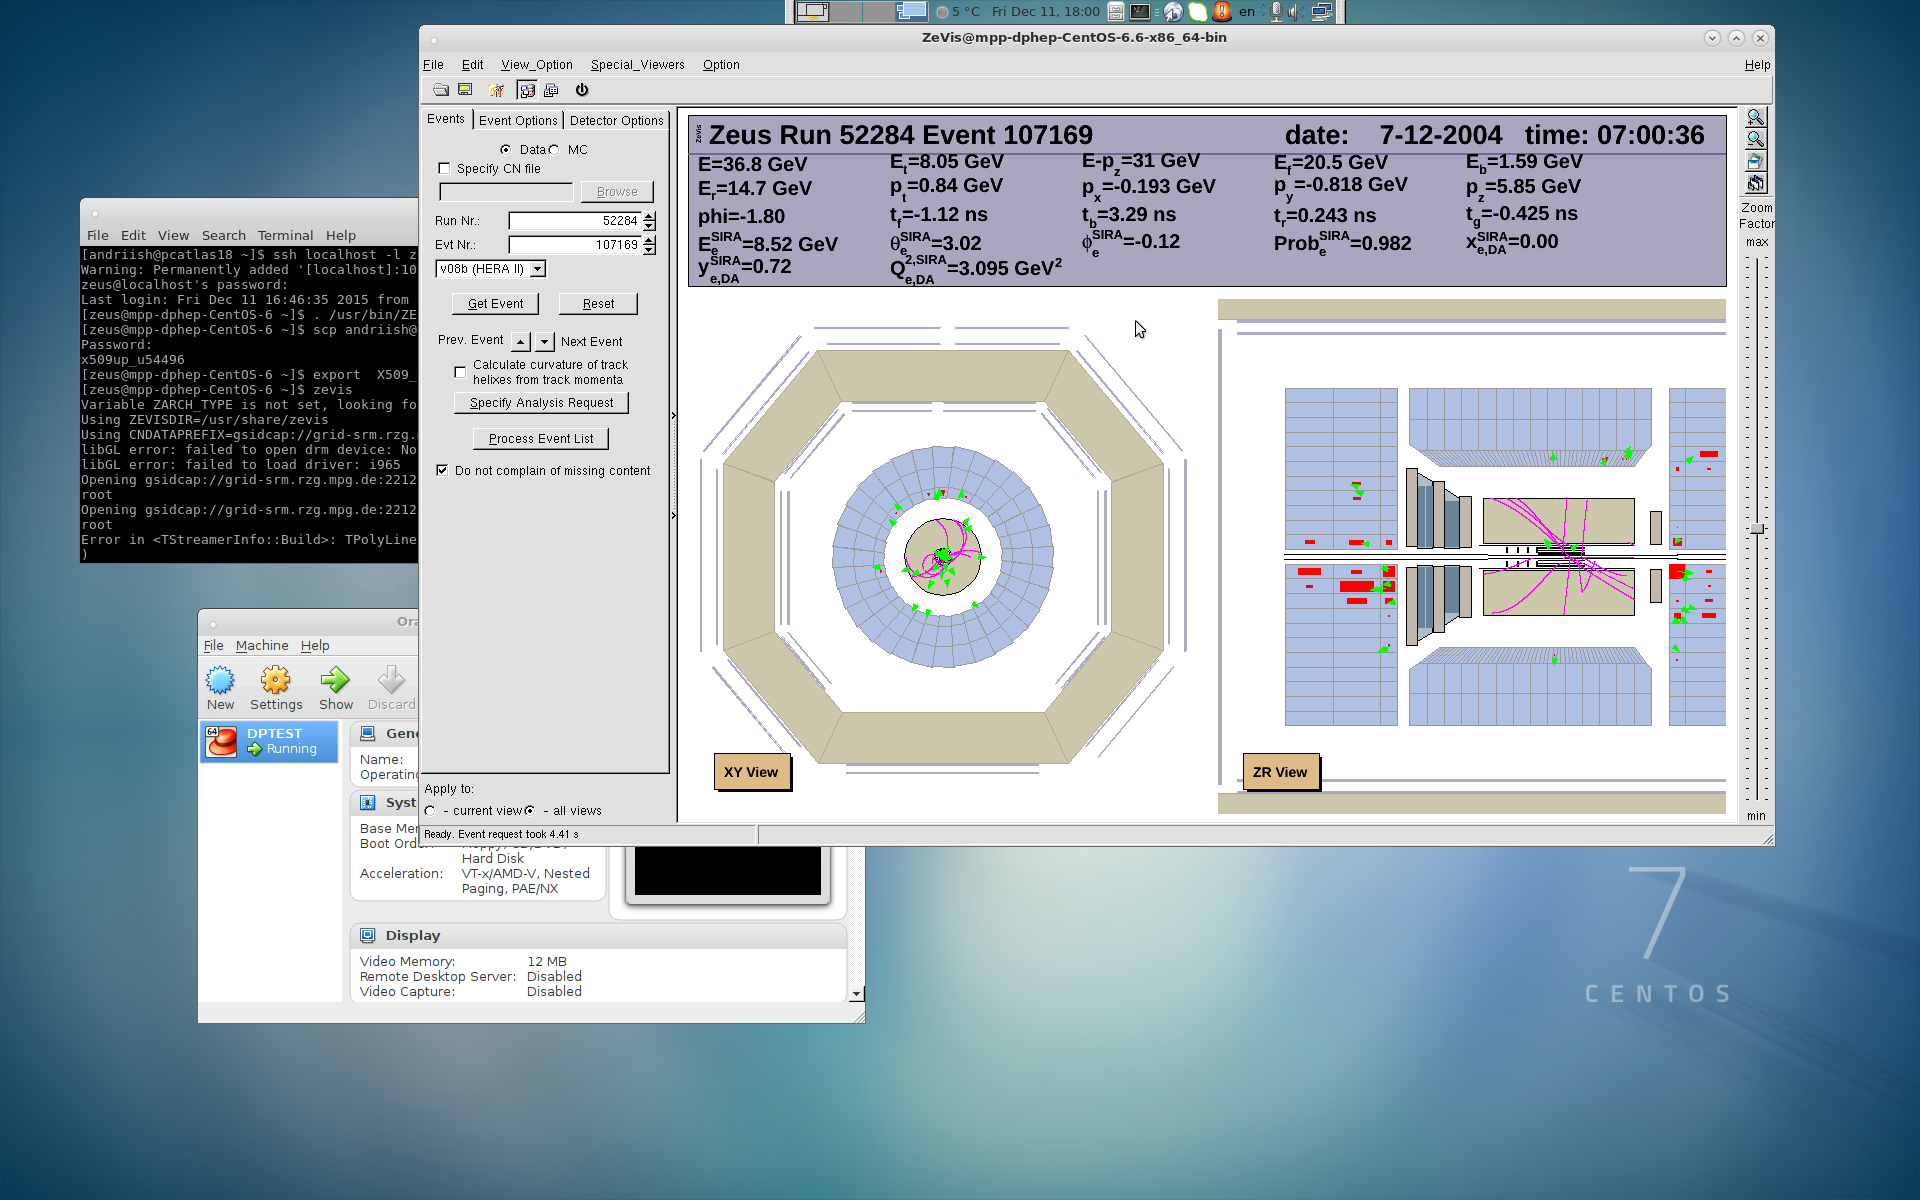
\includegraphics[width=1.0\textwidth]{eps/Screenshot_2.eps}
\end{figure}
}





\frame{\frametitle{The MC recipe ingredients}
\begin{itemize}
\item Instruction to generate events with old JADE generators are prepared.
\item An interface to modern HEP event records based on HepMC3 libray is developed.
  JADE MC  can be produced from with modern MC generator, e.g.\ NLO capable SHERPA+BlackHat.
\item ZMCSP (JADE Monte Carlo Standalone Package) is a tarball with  all the software needed for the reconstruction
of MC simulated events. It has no external dependencies, runs on modern Grid clusters, virtual machine, a laptop.
On the Grid it can produce 50-100M events\footnote{JADE has 360M of data events} per week. 
Supplemented with example of scripts and documentation.
%\item The first two samples were generated this summer. See Iurii's talk.
%It was found that the key to success is to {\bf read and follow the instructions}.
%\item There is a lot of computing resources around, where it is possible to generate even large samples.
%20-50-100M events is NOT a problem. 
%\item In practice the generation with new MC generators is not much complicated, however only tiny samples were produced with
%SHERA 2.2 and blackhat 0.9.9.
\end{itemize}
}

\frame{\frametitle{The MC generation: SHERPA+BlackHat multijet setup}
%\begin{figure}\centering
%\includegraphics[width=0.4\linewidth]{kt.eps}
%\includegraphics[width=0.4\linewidth]{nt.eps}
%\end{figure}
Thrust distribution with SHERPA+BlackHat Monte Carlo simulated and reconstructed  sample.
}



\section{Conclusions}

\frame{\frametitle{MPP Data Preservation summary}
\begin{itemize}
\item Data is accessible in  MPCDF.
\item An option for MC production with new and old MC generators exists for JADE and tested. 
\end{itemize}
}
\section{Data Preservation applications}

\frame{\frametitle{JADE Data Preservation applications}
\begin{itemize}
\item Hodronisation effects.
\item QCD with $b$-quarks and modern theory predictions.
\item \dots
\end{itemize}
}

\section{What other experiments can learn from JADE DP}


\frame{\frametitle{Software}
\begin{itemize}
\item Usage of generic technologies for hardware and OS, i.e. IBM mainframes, AIX is important.
\item High code quality, clarity and stability is a key to succees.
Note: some routines are from 1978, i.e. almost 40 years old. 
Few moden experiments can be sure that more than tiny fraction of their code will behave like that.
\item Design of software is important, even complicated things like event display can survive for 30 years if to use good simple approaches, i.e. graphic primitives in this case.
\item good build system makes porting much easier
\item Standartisation of I/O data formats is important.
\end{itemize}
}

\frame{\frametitle{Data}

\begin{itemize}
\item Compressing the data might look like a good solution, but it is bad. Saving 1Tb of disk space today mean lose of days to read the data back tommorow.
\item Keeping reference data is important.
\item Standartisation of I/O data formats is important.
\item Obvious: EBCDIC is bad.
\end{itemize}
}



\frame{\frametitle{What other experiments can learn from JADE DP: Some anecdotes}
\begin{itemize}
\item one important „calibration“ file, containing the recorded 
  luminosities of each run and fill, was stored on a private account
  and therefore lost when DESY archive was cleaned up
\item   Jan Olsson, when cleaning up his office in ~1997, found an old ASCII-printout of the JADE luminosity file.
  Unfortunately, it was printed on green recycling paper - not suitable for scanning and OCR-ing.
  A secretary at Aachen re-typed it within 4 weeks.
  A checksum routine found (and recovered) only 4 typos.
\item an old version of the original BOSlib 1979 version was found, on
  our request, at the Tokyo computer centre.
\item  Peter Bock, when cleaning out an old lab at the Physics Institute
  at Heidelberg University, found a few 9-track tapes containing
  original JADE MC files which were very valuable for validating
  results of our first re-analyses in ~1997
\end{itemize}
}

\frame{\frametitle{What other experiments can learn from JADE DP: Some anecdotes}
\begin{itemize}
\item first port attempt in 2016 was done with AIX 4.3 machine used as router in MPP.
\item Byte ordering problem is solved in the modern gfortran
\end{itemize}
}


\end{document}

